\chapter{排列组合}

\section{组合数}
\begin{itemize}[leftmargin=\inteval{\myitemleftmargin}pt,itemsep=
   \inteval{\myitemitempsep}pt,topsep=\inteval{\myitemtopsep}pt]
\item 排列数:$ P_n^k=\dfrac{n!}{(n-k)!} $,或者写成$ A_n^k $. 
\item 组合数:$ C_n^k=C_n^{n-k}=\dfrac{n!}{k!(n-k)!},\ 
C_n^k+C_n^{k-1}=C_{n+1}^k $. 
\myfootnote{如果不考虑组合数的实际意义,直接面对$ C_n^k=\dfrac{n!}
    {k!(n-k)!} $,想要证明这一定是个整数并不算太容易。若借助递推关系
    $ C_n^k+C_n^{k-1}=C_{n+1}^k $,则容易证明了,因为$ C_n^1=n,\ C_n^2=
    \dfrac{n(n-1)}{2} $必定是整数,递推的结果也必定是整数。} 

\item 因为阶乘函数增长太快,在大多数编程场景下,阶乘函数允许的自变量的范围很小,\\
$ 13! = 6227020800 >2^{32}-1 = 4294967295$ \ (32bit无符号整数的最大值)  \\
$ 21!\approx 5.109\times 10^{19} >2^{64}-1 \approx  1.845\times 10^{19}$ 
\ (64bit无符号整数的最大值)   \\
$ 35!\approx 1.033\times 10^{40} >2^{128} \approx  3.403\times 10^{38}$ 
\ (32bit浮点数的最大值)  \\
$ 171!\approx 1.241\times 10^{309} >2^{1024} \approx  1.798\times 10^{308}$ 
\ (64bit浮点数的最大值)  \\
所以,直接用数组(数列)存储阶乘的值,至多占用$ 171\times 8 = 1368 $\,Byte
的存储空间,就能满足64bit计算的需求。不仅速度快,而且没有多次浮点乘法带来
的累积误差,是一般的编程场景下的最优方案。

\item 对于排列数$P_n^k$和组合数$C_n^k$,在编程计算的时候,最好按$k$和$n$的大小分段实现:
当$k$很小时(比如$k<10$),直接用循环语句实现;当$k$稍大一些时,若$n<171$,使用查询
存储阶乘值的数组的方法实现;若$n\geq 171$,使用先求对数再求指数的方法,即
\begin{gather*}
    P_n^k=\exp{\left(\ln \dfrac{n!}{(n-k)!}\right)}=\exp{(\ln(n!)-\ln((n-k)!))} \\
    C_n^k=\exp{\left(\ln \dfrac{n!}{k!(n-k)!}\right)}=\exp{(\ln(n!)-\ln(k!)-\ln((n-k)!))}
\end{gather*}
其中$\exp()$表示以e为底的指数函数,阶乘的对数$\ln(n!)$有专门的计算方法
(利用Stirling公式),不用担心因$n!$过大导致无法计算。
    
\item 二项式定理:$ (a+b)^n=\sum\limits_{k=0}^nC_n^ka^kb^{n-k}=
\sum\limits_{k=0}^nC_n^ka^{n-k}b^k $ .
\item 几个多项展开式:
\begin{align*}
    (a+b+c)^2 &=a^2+b^2+c^2+2(ab+ac+bc) \\
    (a+b+c)^3 &=a^3+b^3+c^3+3(a^2b+ab^2+b^2c+bc^2+a^2c+ac^2)+6abc \\
    (a+b+c)^4 &=a^4+b^4+c^4+4(a^3b+ab^3+b^3c+bc^3+a^3c+ac^3) \\
    &+6(a^2b^2+b^2c^2+a^2c^2)+12(a^2bc+ab^2c+abc^2) \\
    (a+b+c+d)^2 &=a^2+b^2+c^2+d^2+2(ab+ac+ad+bc+bd+cd) 
\end{align*}
\item 杨辉三角:左右对称性,内部元素等于肩上两数之和,
每行的和构成公比为2的等比数列,每行奇数项的和等于偶数项的和,
杨辉三角还包含了斐波那契数列。
\begin{align*}
    F_1=&\  C_0^0=1 \\
    F_2=&\  C_1^0=1 \\
    F_3=&\  C_2^0+C_1^1=2 \\
    F_4=&\  C_3^0+C_2^1=3 \\
    F_5=&\  C_4^0+C_3^1+C_2^2=5 \\
    F_6=&\  C_5^0+C_4^1+C_3^2=8 \\
    F_7=&\  C_6^0+C_5^1+C_4^2+C_3^3=13 \\
    F_8=&\  C_7^0+C_6^1+C_5^2+C_4^3=21 \\ 
    &\cdots \\
    F_n=&\  C_{n-1}^0+C_{n-2}^1+\cdots+C_{n-1-m}^m\quad \left(m=\left\lfloor
    \frac{n-1}{2} \right\rfloor\right)   
\end{align*}
其中,$ \lfloor x \rfloor $表示向下取整,即不超过$ x $的最大整数,比如
$ \lfloor 4.3 \rfloor=4,\ \lfloor 6.9 \rfloor=6 $. 
\item 加法原理(分类),乘法原理(分步)。
\item 德摩根(De Morgan)定律:$ \overline{A \cap B}=\overline{A}\cup 
\overline{B},\ \overline{A \cup B}=\overline{A}\cap \overline{B} $. 
同一个等式中必定有一个交集符号,一个并集符号。
%\begin{align*}
%	f(x)=(1+x)^n=\sum_{k=0}^{n} C_n^k x^k 
%\end{align*}

\begin{table}[h] 
\caption{组合恒等式} 
\centering
\begin{tabular}{l|l} \label{组合恒等式}
    $\sum\limits_{k=r}^{n} C_k^r=C_{n+1}^{r+1}=C_n^r+C_n^{r+1}$  &		
    $\sum\limits_{k=0}^{r}C_m^kC_n^{r-k}=C_{n+m}^r $     \\
    $\sum\limits_{k=0}^{n} C_n^k=2^{n} $		&
    $\sum\limits_{k=1}^{n} kC_n^k=n\cdot2^{n-1} $  \\
    $\sum\limits_{k=1}^{n} k^2C_n^k=n(n+1)\cdot2^{n-2} $  &
    $\sum\limits_{k=0}^{n} C_{2n}^k=2^{2n-1}+\dfrac{(2n)!}{2(n!)^2} $  \\
    $\sum\limits_{k=0}^{n} \left( C_{n}^k\right) ^2=\dfrac{(2n)!}{(n!)^2} $  &
    $C_n^kC_k^r=C_n^rC_{n-r}^{k-r} $
\end{tabular}
\end{table} 
% \vspace{0.5cm}
\item 含有$ n $个元素的集合的子集(包括空集和全集)的数量为
$ 2^n $,即$\sum\limits_{k=0}^{n} C_n^k=2^{n} $. 也可以认为每个元素都有
选出或不选出2种可能,
所以总共有$2\times 2\times \cdots\times 2= 2^n $种选法。

\item 求证:$ \sum\limits_{k=1}^{n} kC_n^k=n\cdot2^{n-1} $. \\
\textbf{方法一} 
\begin{gather*}
    kC_n^k=k\dfrac{n!}{k!(n-k)!}=n\dfrac{(n-1)!}{(k-1)![(n-1)-(k-1)]!}=nC_{n-1}^{k-1} 	
\end{gather*}
\begin{gather*}
    \sum_{k=1}^{n} kC_n^k=\sum_{k=1}^{n} nC_{n-1}^{k-1}=n\sum_{k=1}^{n} C_{n-1}^{k-1}
    =n\cdot 2^{n-1}
\end{gather*}
\textbf{方法二}
\begin{align*}
    (1+x)^n=C_n^0+C_n^1x+C_n^2x^2+\cdots + C_n^nx^n
\end{align*}
对$ x $求导:
\begin{align} \label{二项展开式两边求导}
    n(1+x)^{n-1}=C_n^1+2C_n^2x+\cdots + nC_n^nx^{n-1}
\end{align}
令$ x=1 $即可。\\
\textbf{方法三}\ 倒序相加:
\begin{align*}
    S_n=&\ C_n^0+C_n^1+2C_n^2+\cdots+(n-2)C_n^{n-2} +(n-1)C_n^{n-1}+ nC_n^n \\
    S_n=&\ nC_n^n+(n-1)C_n^{n-1}+(n-2)C_n^{n-2}+\cdots+2C_n^2+ C_n^1 +C_n^0 \\
    2S_n=&\ n(C_n^0+C_n^1+\cdots +C_{n-1}^1+C_n^n)=n\cdot 2^n \\
    S_n=&\  n\cdot 2^{n-1}
\end{align*}

\item 在等式$ (1+x)^n=C_n^0+C_n^1x+C_n^2x^2+\cdots + C_n^nx^n $
中令$ x=\i $\ (虚数单位),则
\begin{align*}
    (1+\i)^n=&\ C_n^0+C_n^1\i+C_n^2\i^2+C_n^3\i^3+
    \cdots + C_n^n\i^n  \\
    =&\ C_n^0+C_n^1\i-C_n^2-C_n^3\i+
    \cdots + C_n^n\i^n  \\
    =&\ (C_n^0-C_n^2+C_n^4-\cdots)+\i (C_n^1-C_n^3+C_n^5-\cdots)
\end{align*}
因为$ 1+\i=\sqrt{2}\left(\cos\dfrac{\pi}{4}+
\i\sin\dfrac{\pi}{4}\right) $,利用\eqref{欧拉公式n倍角情形}式,
有$ (1+\i)^{n}=\sqrt{2^{n}}\left(\cos\dfrac{n\pi}{4}
+\i\sin\dfrac{n\pi}{4}\right) $,于是
\begin{align*}
    (1+\i)^{n}
    =&\ (C_n^0-C_n^2+C_n^4-\cdots)+\i (C_n^1-C_n^3+C_n^5-\cdots)\\
    =&\ \sqrt{2^{n}}\cos\dfrac{n\pi}{4}
    +\i\sqrt{2^{n}}\sin\dfrac{n\pi}{4}
\end{align*}
比较实部和虚部就能得到两个等式:
\begin{gather*}
    C_n^0-C_n^2+C_n^4-\cdots=\sqrt{2^{n}}\cos\dfrac{n\pi}{4} \\
    C_n^1-C_n^3+C_n^5-\cdots=\sqrt{2^{n}}\sin\dfrac{n\pi}{4}
\end{gather*}

\item 正整数的分拆是指将一个正整数分成几个正整数的和。即
\begin{align*}
    n=n_1+n_2+\cdots n_k \quad (n_i>0,\ 1\leq i\leq k)
\end{align*}
$ n_i $叫做该分拆的分部量。如果将各个$ n_i $任意交换位置后,仍然视为同一种表示法,
这样的分拆叫做无序分拆,否则称之为有序分拆。
对于有序分拆,可以视为排成一行的$ n $件物品,向它们的$ n-1 $个
间隔中插入$ k-1 $块隔板,将物品分成$ k $组,所以有序分拆的方法数为$ C_{n-1}^{k-1} $. 
无序分拆比较复杂,可查阅许胤龙、孙淑玲编著的《组合数学引论》。

\item\label{容斥原理} 容斥原理:以两种性质A和B为例,
在一个集合中,假设具有性质A的元素的个数为$ n_A $,
具有性质B的元素的个数为$ n_B $,同时具有性质$ A $和$ B $的元素的
个数为$ n_{AB} $,那么具有性质A或B的元素个数是$ n_A+n_B-n_{AB} $.
请结合下图理解:
\begin{figure}[H]
    \centering
    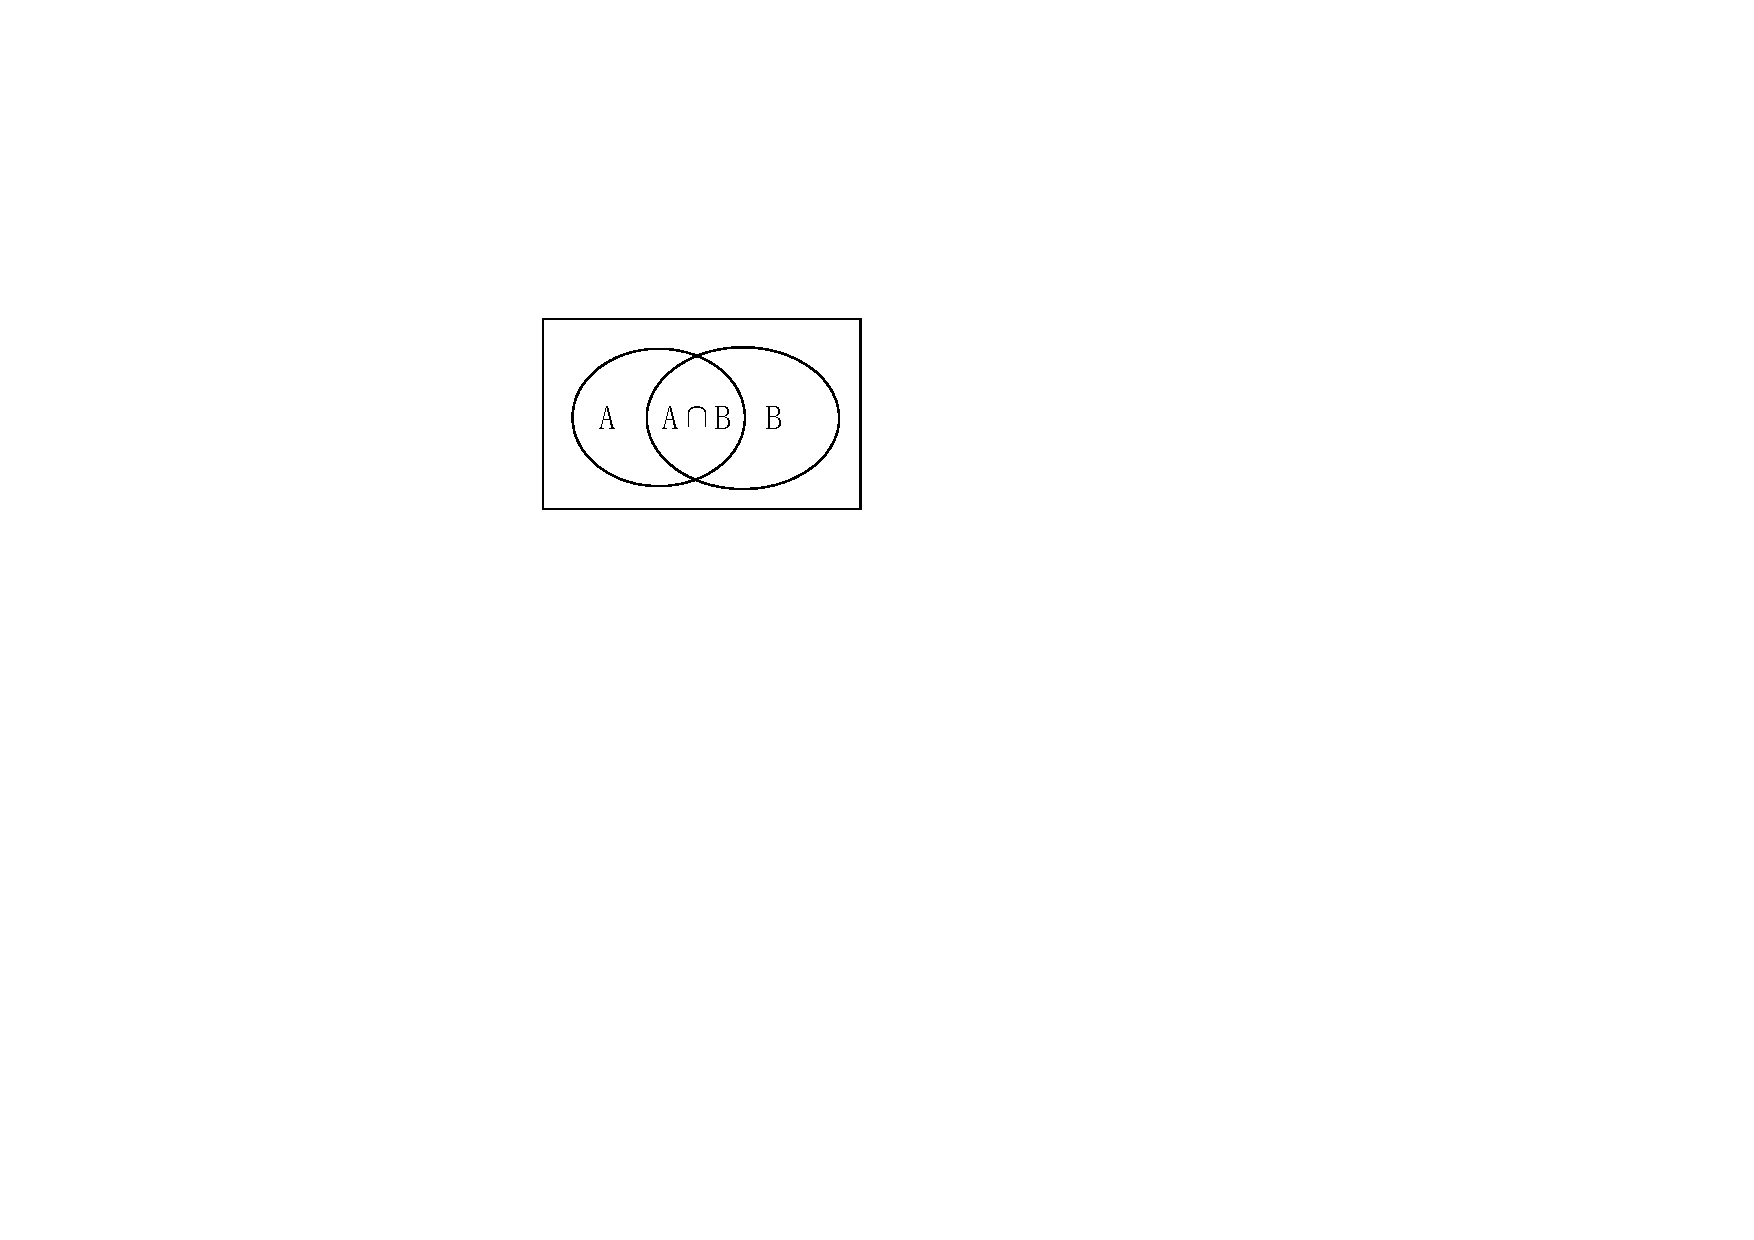
\includegraphics[width=0.3\linewidth]{PDF_Picture/韦恩图-交集}
\end{figure}
我们通过一个具体的例子来理解容斥原理。
两个正整数互质(互素)是指两个数的最大公因子是1
(所以1与任何正整数都是互质的),
考虑小于等于28且与28互质的正整数的个数,
不过,直接考虑互质的数会比较麻烦,
让我们考虑小于等于28且与28不互质的数。
28的质因子是2和7,28以内所有2的倍数和7的倍数
都与28不互质,2的倍数有14个,
7的倍数有4个,能不能说2的倍数或7的倍数一共$ 14+4=18 $个呢?
不能!因为14和28都既是2的倍数、又是7的倍数,刚刚被算了2次,
得减掉,于是2的倍数或7的倍数一共$ 14+4-2=16 $个,互质的数的
个数就是$ 28-16=12 $,这12个数依次是1,3,5,9,11,13,15,17,
19,23,25,27. 请读者按上面的方法说明,小于等于30且与30互质的
数的个数是8\footnote{这8个数依次是$ 1,7,11,13,17,19,23,29 $.\q 
    8又恰好是一个字节对应的bit数,这个性质可以用来实现一个巧妙的算法,
    参见本书作者写的文章《30个整数映射到1个字节,
    查表法实现小范围内常数时间素性判定》\\
    https://zhuanlan.zhihu.com/p/19939334005 }.

\item 小于等于$ n $且与$ n $互质的正整数的
个数被定义为欧拉函数$ \varphi(n) $. 
若$ p,q $ 都是质数且不相等,$ k $是正整数,则
$ \varphi(p)=p-1 $,$ \varphi(pq)=pq-p-q+1=(p-1)(q-1) $,
$ \varphi(p^k)=p^k-p^{k-1}=p^{k-1}(p-1) $.

\item 正整数$ n $可以分解成其质因子的幂的乘积的形式,
$ n=p_1^{e_1}p_2^{e_2}\cdots p_k^{e_k} $,比如
$ 28=2^2\times 7,\ 30=2\times 3\times 5,\ 12375=3^2\times 5^3 \times 11 $,
那么
\begin{gather}\label{eulerPhi函数的计算公式}
    \varphi(n)=n\left(1-\dfrac{1}{p_1}\right)
    \left(1-\dfrac{1}{p_2}\right)\cdots \left(1-\dfrac{1}{p_k}\right)
\end{gather}
比如
\begin{align*}
    \varphi(28)&=28\left(1-\dfrac{1}{2}\right)\left(1-
    \dfrac{1}{7}\right) \\
    &=28\left(1-\dfrac{1}{2}-\dfrac{1}{7}+\dfrac{1}{2\times 7}\right) \\
    &=28-\left(\dfrac{28}{2}+\dfrac{28}{7}-\dfrac{28}{2\times 7}
    \right)=12 \\
    \varphi(30)&=30\left(1-\dfrac{1}{2}\right)
    \left(1-\dfrac{1}{3}\right)\left(1-\dfrac{1}{5}\right) \\
    &=30\left(1-\dfrac{1}{2}-\dfrac{1}{3}-\dfrac{1}{5}+
    \dfrac{1}{2\times 3}+\dfrac{1}{2\times 5}+\dfrac{1}{3\times 5}
    -\dfrac{1}{2\times 3\times 5}\right) \\
    &=30-\left(\dfrac{30}{2}+\dfrac{30}{3}+\dfrac{30}{5}-
    \dfrac{30}{2\times 3}-\dfrac{30}{2\times 5}-\dfrac{30}{3\times 5}
    +\dfrac{30}{2\times 3\times 5}\right)
    =8
\end{align*}

\item 有$ n $级台阶,每次只允许上1级或2级,总共有多少种走法?\\
\textbf{解}\ 该问题可视为正整数$ n $的有序分拆,同时要求所有的分部量小于等于2,
但直接使用隔板法,会面临无法限制分部量的大小的问题。
现改为寻找递推关系:到达第$ n $级台阶,
可能是从$ n-2 $级台阶上2级到达的,也可能是从$ n-1 $级台阶上1级到达的,令$ F_n $
代表上$ n $级台阶的方法数,那么$ F_n=F_{n-1}+F_{n-2} $,这正是斐波那契数列
的递推关系,$ F_1=1,\ F_2=2 $,相当于常规的斐波那契数列($ F_1=1,F_2=1 $)从
第2项开始。

\item 汉诺塔问题:现有A、B、C三根立柱以及$ n $个大小不等的中空圆盘,
这些圆盘从小到大套在A柱上形成一座塔,要求把$ n $个圆盘从A柱上搬到C柱上,
并仍然保持下大上小的顺序。要求每次只能从一根立柱上拿下一个圆盘放到另外一根
立柱上,且不允许大盘压在小盘上,至少要搬多少次?\\
\textbf{解}\ 设$ H(n) $表示有$ n $个圆盘时最小的搬动次数,整个搬动过程可
分成三个阶段:\\
I.将套在A柱上面的$ n-1 $个圆盘从A柱搬到B柱,搬动次数为$ H(n-1) $;\\
II.把A柱最下面的圆盘搬到C柱上,搬动次数为1;\\
III.把B柱上的$ n-1 $个圆盘搬到C柱上,搬动次数为$ H(n-1) $;\\
于是递推关系为:$ H(n)=2H(n-1)+1 $,初始条件为$ H(1)=1 $. 因为
\begin{align*}
    H(n)+1=2[H(n-1)+1]=2^2[H(n-2)+1]=\cdots=2^{n-1}[H(1)+1]=2^n
\end{align*}
所以,$ H(n)=2^n-1 $. 

\item 令数列 $ \{ a_k \} (1\leq k \leq n) $是集合
$ \{ 1,2,\cdots n \} $的一个排列,
如果每个元素都不在其对应下标的位置上,即$ a_k\neq k $,
那么这种排列称为错位排列,或错排。1 2 3 4的错排有:
\begin{table}[h]
    \centering
    \begin{tabular}{ccc}
        4 3 2 1 & 4 3 1 2 & 4 1 2 3 \\
        3 4 2 1 & 3 4 1 2 & 3 1 4 2 \\
        2 1 4 3 & 2 3 4 1 & 2 4 1 3 
    \end{tabular}
\end{table} \\
设$ n $个元素错排的方案数为$ D_n $,第一步,考虑元素$ a_n $,
把它放在除$ n $位以外的某个位置,比如位置$ k $,
一共有$ n-1 $种放法;第二步,考虑元素$ a_k $,这时有两种情况:
(1)把它放到位置$ n $,此时$ k,n $两个位置分别被$ a_n,a_k $占据,
已经错位了,那么剩下$ n-2 $个元素错排即可,有$ D_{n-2} $种排法;
(2)元素$ a_k $不放到位置$ n $(可把元素$ a_k $想象成不能出现在
第$ n $位的一个新的$ a_n $),这时对除$ a_n $以外的$ n-1 $
个元素错排,有$ D_{n-1} $种排法。根据乘法和加法原理,
$ D_n=(n-1)(D_{n-1}+D_{n-2}),\ D_1=0,\ D_2=1. $
\begin{gather*}
    D_n-nD_{n-1}=(-1)[D_{n-1}-(n-1)D_{n-2}]=\cdots =(-1)^{n-2}[D_2-D_1]=(-1)^n 
\end{gather*}
首尾同除$ n! $,
\begin{gather*}
    \dfrac{D_n}{n!}-\dfrac{D_{n-1}}{(n-1)!}=\dfrac{(-1)^n}{n!} 
\end{gather*}
取$ n-1 $个这样的式子相加:
\begin{align}\label{错排通项公式}
    D_n=n!\left[ 1-\dfrac{1}{1!}+\dfrac{1}{2!}-\cdots 
    +(-1)^n\dfrac{1}{n!}\right] 
\end{align}
上式也可用数学归纳法证明。

上面介绍的上台阶、汉诺塔和错排三个问题,如果试图直接寻找答案,无疑是相当困难的,而寻找递推关系则要简单得多。
%常考题型,对$ \left(ax^{\alpha}+by^{\beta} \right)^n $的展开式,求所有系数的和,奇数项系数的和,
%偶数项系数的和,所有系数绝对值的和,常数项。方法:令$ x,y=-1,0,1 $这三个特殊值,以及令
%$ ax^{\alpha}+by^{\beta} =0 $. \\
%\item \  
% $ (2x+3x^2)^6=c_0+c_1 $
% 另一类问题是,
\item $ \left(ax^{\alpha}+bx^{\beta} \right)^n $的展开式的通项为
$ T_{r+1}=C_n^ra^{n-r}b^rx^{(n-r)\alpha+r\beta} $,
设$ C_n^m a^{n-m}b^m $是最大的系数,则
\begin{align}\label{二项式系数最大值不等式组-首次出现}
    \left\{
    \begin{aligned}
        & C_n^m a^{n-m}b^m\geq C_n^{m-1} a^{n-m+1}b^{m-1} \\
        & C_n^m a^{n-m}b^m\geq C_n^{m+1} a^{n-m-1}b^{m+1}
    \end{aligned}
    \right.
\end{align} 
\begin{align*}
    \left\{
    \begin{aligned}
        \dfrac{b}{m}   \geq &\ \dfrac{a}{n-m+1} \\
        \dfrac{a}{n-m} \geq &\ \dfrac{b}{m+1}
    \end{aligned}
    \right. \quad \Rightarrow \quad 
    \dfrac{bn-a}{a+b} \leq m \leq \dfrac{bn+b}{a+b}
\end{align*} 
因为$ \dfrac{bn-a}{a+b}+1=\dfrac{bn+b}{a+b} $,所以不等式组一定有解。
当$ \dfrac{bn-a}{a+b} $为整数时,有两个解;否则只有一个解。例如,
$ (2x+5x^2)^{12} $展开式中系数最大的项是
$ C_{12}^{3}(2x)^3(5x^2)^9=3437500000x^{21} $,所有系数的图像如下
\footnote{对于高考中允许使用计算器的省份,则可以直接使用计算器的表格(Table)功能,
    定义$ f(x)= 12Cx\times 2^{12-x}\times 5^x,\ x=0\sim 12 $即可。}:
% plot(fliplr(coeffs(expand((2*x+5*x^2)^12))),'k.','markersize',20);
% axis([0 14 -10^8 3.6*10^9]);grid on
\begin{figure}[h]
    \centering
    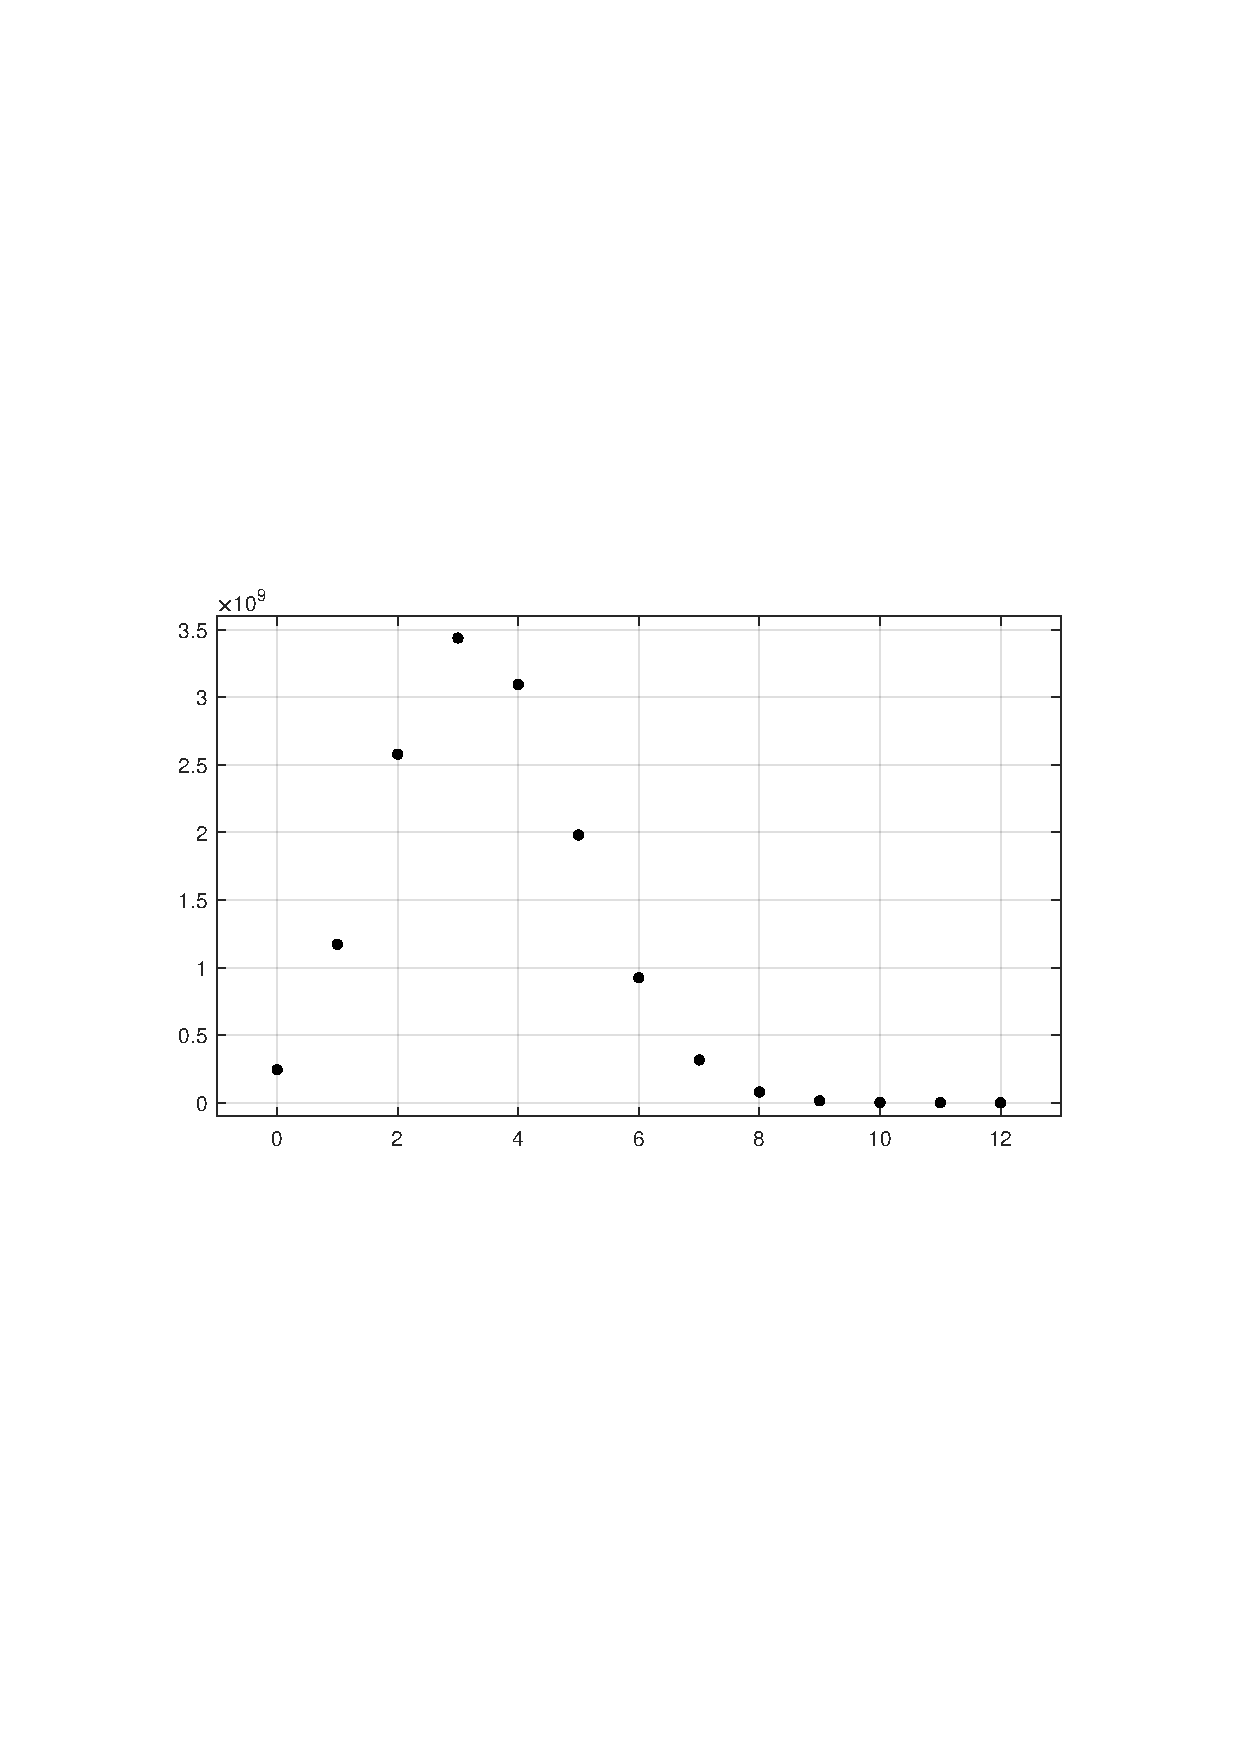
\includegraphics[width=0.5\linewidth]{二项式系数最大}
\end{figure} 

\item 设随机变量$ X $服从二项分布$ b(n,p) $,每次实验时,事件$ A $发生的概率为
$ p $,那么在$ n $次实验中事件$ A $发生$ k $次的概率为
\begin{align*}
    P\{X=k\}=C_n^kp^k(1-p)^{n-k}
\end{align*}
若想找出$ k $为何值时概率最大,可采用与不等式组(\ref{二项式系数最大值不等式组-首次出现})
一样的方法,可解得:
\begin{align*}
    (n+1)p-1\leq k \leq (n+1)p 
\end{align*}


\item $^*$ 一个正方形无法划分为奇数个面积相等的三角形
\footnote{参见 Paul Monsky, On dividing a square into triangles, Amer. Math. Monthly 77 (1970), no. 2, 161–164. 或者参见 https://zhuanlan.zhihu.com/p/398055396 . }。

\item $^*$ 设$ f(x) $在区间$ [0,1] $上连续不断,则多项式
\begin{gather*}
    \sum_{k=0}^{n}f\left(\dfrac{k}{n}\right)C_n^kx^k(1-x)^{n-k}
\end{gather*}
被称为伯恩斯坦(Bernstein)多项式,当$ n $增大时,该多项式可以越来越接近$ f(x) $本身。

\item $^*$ 在核磁共振(Nuclear Magnetic Resonance,NMR)现象中,当一个氢原子核有$ n $
个临近的全同氢原子核存在时,其NMR吸收峰分裂为$ n+1 $个,各峰的强度之比为$ 
C_n^0:C_n^1:C_n^2:\cdots :C_n^n $,该规律被称为自旋裂分$ n+1 $规律。

\item $^*$ 计算任意烷烃$ \mathrm{C_nH_{2n+2},\ n}\in \textbf{N}^+ $
的同分异构体数量是一个比较困难但意义不大的问题,当$ n=1\sim 10 $时,
同分异构体数量依次为1,1,1,2,3,5,9,18,35,75.目前只能递推计算,找不出通项公式。

\end{itemize}

\section{例题}
\begin{enumerate}[label={【\textbf{例\thechapter.\arabic*}】},
 leftmargin=\inteval{\myenumleftmargin}pt,
 itemsep=\inteval{\myenumitempsep}pt,
 itemindent=\inteval{\myenumitemindent}pt]
\item 到四面体的四个顶点距离相等的平面个数是多少? 
\begin{figure}[h]
    \centering
    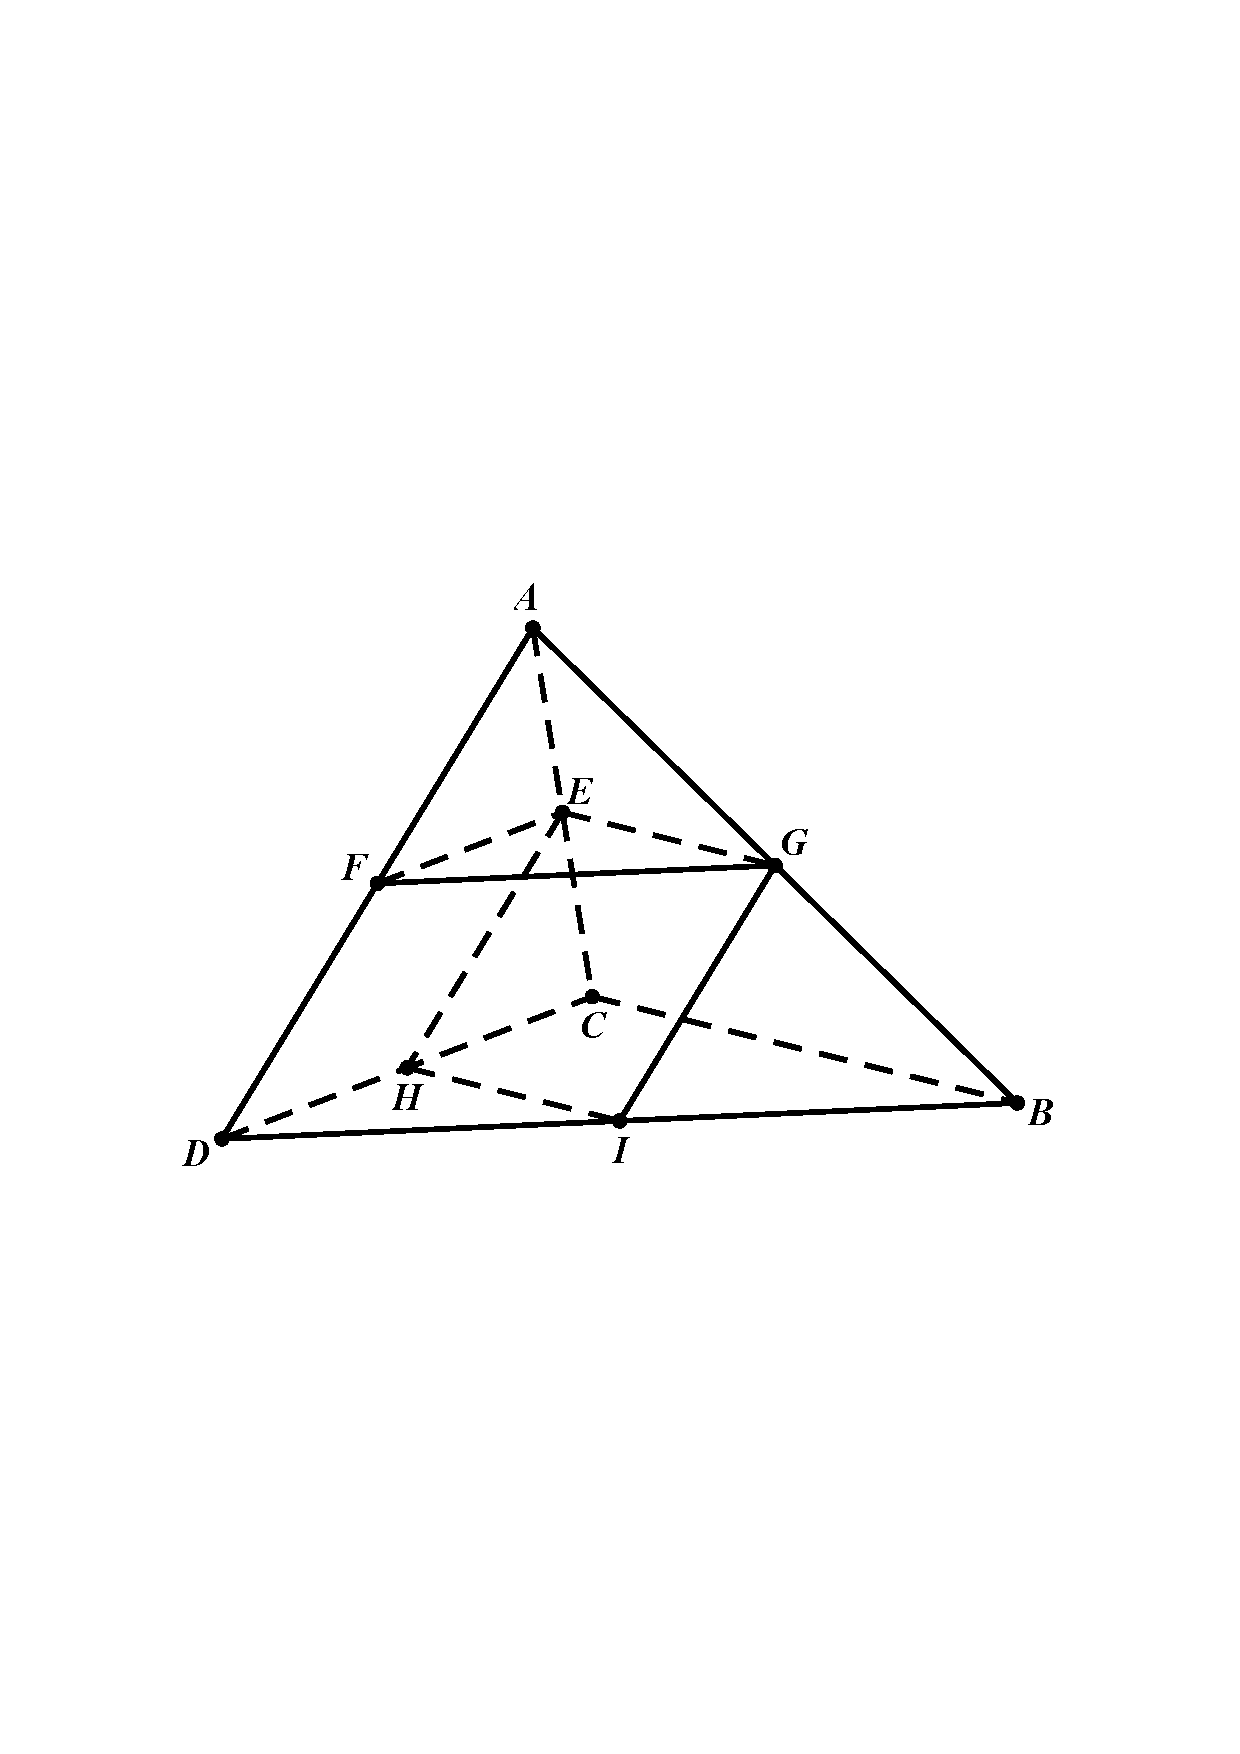
\includegraphics[width=0.4\linewidth]{四面体_中位面}
\end{figure} \\
\textbf{解}\ 共用同一个顶点的三条棱的中点确定了一个三角形,称为四面体的中位面,
比如$ \Delta EFG $,中位面到4个顶点的距离都相等。(1)四面体一共有4张不同的中位面;
(2)取特定的4条棱的中点,比如$ EHIG $,有3种不同取法。
故一共有7张不同平面到四个顶点距离相等。\\
\textbf{注}:$ S_{\Delta EFG}=\dfrac{1}{4}S_{\Delta CDB},\ 
V_{A-EFG}=\dfrac{1}{8}V_{A-CDB} $. 

\item 四面体的顶点与棱的中点共10个点,在其中取4个不共面的点,
有多少种不同的取法?\\
\textbf{解}\ 10个点中任取4点,有$ C_{10}^4=210 $种取法。考虑4点共面的情况:
(1)4点在四面体的同一个面上,
有$ 4C_6^4=60 $种;(2)4点中3点在同一条棱上(比如$ A,E,C $),剩下一点在对棱中点上
(比如$ I $),有6种;(3)同上一道例题的情形(2),有3种。
所以,不共面的取法有$ 210-60-6-3=141 $种。

\item 将5名志愿者分配到3个不同的奥运场馆参加接待工作,
每个场馆至少分到一名志愿者的方案有 $ 
C_5^3P_3^3+\dfrac{C_5^2C_3^2}{P_2^2}P_3^3=150 $种。(平均分组)

\item 有10个翻译,其中3人只能译英语,2人只能译法语,另5人既能译英语又能译法语,现欲从中
选取2名英语3名法语翻译,有几种选法?\\
\textbf{解}\ 针对既能翻译英语又能翻译法语的5人进行分类:

5人中选1人译法语,有$ C_5^1C_2^2C_7^2 = 105 $种选法;

5人中选2人译法语,有$ C_5^2C_2^1C_6^2 = 300 $种选法;

5人中选3人译法语,有$ C_5^3C_5^2= 100 $种选法; \\
所以共有$ 105 + 300 + 100 = 505 $种选法。(请按5人中选1人和2人译英语的分类方法再算一遍。)

\item 马路上有编号为1,2,3,…,10的十盏路灯,为节约用电又不影响照明,可以把其中3盏灯关掉,
但不可以同时关掉相邻的两盏或三盏,在两端的灯都不能关掉的情况下,有多少种不同的关灯方法?\\
\textbf{解}\ (插空法,也称隔板法)本题等价于在7只亮着的路灯之间的6个空档中插入3只
熄掉的灯,故所求方法总数为$  C_6^3= 20 $种方法。

\item 下图的矩形由$ 3\times 5 $个正方形组成,则从$ M $点到$ N $点
的最短路径有多少种?
\begin{figure}[h]
    \centering
    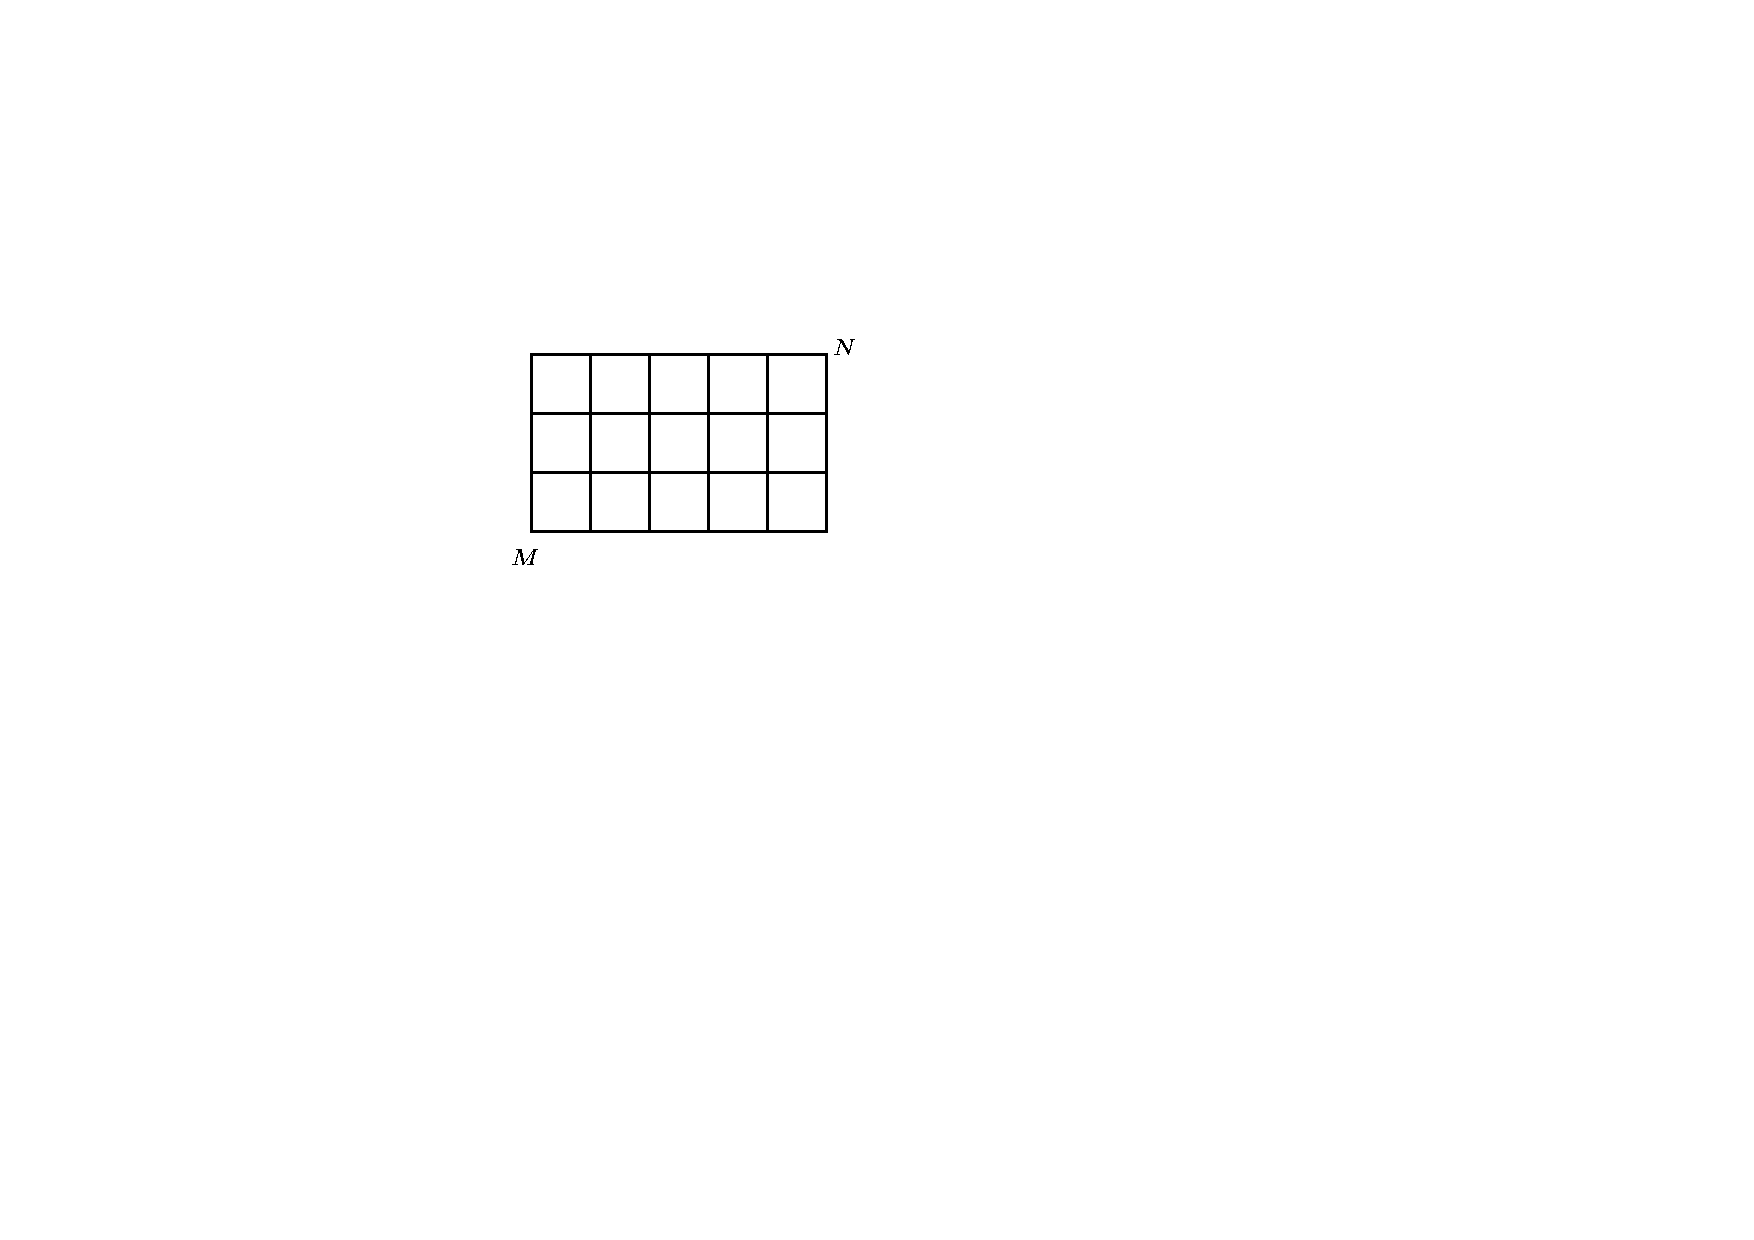
\includegraphics[width=0.3\linewidth]{正方形网格走对角顶点}
\end{figure} \\
\textbf{解}\ 从$ M $到$ N $必须向上走3步,向右走5步,共走8步。
只要从8步中选出3步向上走(或者5步向右走),就可以确定一种走法,所以答案为
$ C_8^3=C_8^5=56 $.

\item \label{偶数件物品选奇数件是偶数} 
求证:从偶数件不同物品中选出奇数件物品的方法数总是偶数。即
$ C_{2n}^1 $,$ C_{2n}^3 $,$ C_{2n}^5,\cdots $都是偶数。\\
\textbf{证}\ $ C_{2n}^1=2n $显然是偶数,而且$ C_4^1=C_4^3=4 $是偶数,
那么只需证明$ C_{2n}^{2m-1} $是偶数,其中$ n\geq 3,\ 2\leq m\leq n $. 
固定$ m $,对$ n $用数学归纳法,并利用组合数的递推关系,
\begin{align*}
    C_{2n}^{2m-1} &=C_{2n-1}^{2m-2}+C_{2n-1}^{2m-1} \\
    &=(C_{2n-2}^{2m-3}+C_{2n-2}^{2m-2})+(C_{2n-2}^{2m-2}+C_{2n-2}^{2m-1}) \\
    &=\underbrace{C_{2n-2}^{2m-3}}_{\text{偶数}}+
    \underbrace{C_{2n-2}^{2m-1}}_{\text{偶数}}+
    \underbrace{2C_{2n-2}^{2m-2}}_{\text{偶数}}
\end{align*}

\item $^*$ 观察下列等式:
\begin{align*}
    &(\sqrt{2} \pm 1)^{1}=\sqrt{2} \pm \sqrt{1} \\
    &(\sqrt{2} \pm 1)^{2}=3 \pm 2\sqrt{2}=\sqrt{9} \pm \sqrt{8} \\
    &(\sqrt{2} \pm 1)^{3}=5\sqrt{2} \pm 7=\sqrt{50} \pm \sqrt{49} \\
    &(\sqrt{2} \pm 1)^{4}=17 \pm 12\sqrt{2}=\sqrt{289} \pm \sqrt{288} \\
    & \q\q \vdots \\
    &(\sqrt{3} \pm \sqrt{2})^{1}=\sqrt{3} \pm \sqrt{2} \\
    &(\sqrt{3} \pm \sqrt{2})^{2}=5 \pm 2\sqrt{6}=\sqrt{25} \pm \sqrt{24} \\
    &(\sqrt{3} \pm \sqrt{2})^{3}=9\sqrt{3} \pm 11\sqrt{2}=\sqrt{243} \pm 
    \sqrt{242} \\
    &(\sqrt{3} \pm \sqrt{2})^{4}=49 \pm 20\sqrt{6}=\sqrt{2401} \pm \sqrt{2400}    
\end{align*}
求证:$ (\sqrt{n}\pm\sqrt{n-1})^k=\sqrt{N}\pm\sqrt{N-1} $,
$ n,k,N\in \textbf{N}^+ $. \\
\textbf{证}\ 以$ (\sqrt{n}+\sqrt{n-1})^{k} $
为例(当加号情形成立时,减号情形自动成立),对$ k $用数学归纳法,
假设$ (\sqrt{n}+\sqrt{n-1})^k=\sqrt{N}+\sqrt{N-1} $成立,
当$ k $变成$ k+1 $时,
\begin{align*}
    (\sqrt{n}+\sqrt{n-1})^{k+1}&=(\sqrt{N}+\sqrt{N-1})(\sqrt{n}+\sqrt{n-1}) \\
    &=\sqrt{Nn}+\sqrt{N(n-1)}+\sqrt{n(N-1)}+\sqrt{(N-1)(n-1)}
\end{align*}
我们希望上式具有$ \sqrt{M}+\sqrt{M-1}\ (M\in \textbf{N}^+) $的形式,
依据上面的数值例子,有
\begin{align}
    \sqrt{Nn}+\sqrt{(N-1)(n-1)} &=\sqrt{M}   \label{sqrtn1} \\
    \sqrt{N(n-1)}+\sqrt{n(N-1)} &=\sqrt{M-1} \label{sqrtn2}
\end{align}
两边平方,
\begin{align}
    Nn+2\sqrt{Nn(N-1)(n-1)}+Nn-(N+n)+1 &=M   \label{sqrtn3} \\
    Nn-N+2\sqrt{Nn(N-1)(n-1)}+Nn-n     &=M-1 \label{sqrtn4}
\end{align}
可以发现(\ref{sqrtn3})式和(\ref{sqrtn4})式是等价的,那么
只需证明$ \sqrt{Nn(N-1)(n-1)} $是整数,由二项式定理和归纳假设,
\begin{align*}
    \sqrt{N} &=\dfrac{1}{2}\left[(\sqrt{n}+\sqrt{n-1})^k
    +(\sqrt{n}-\sqrt{n-1})^k\right] \\
    \sqrt{N-1} &=\dfrac{1}{2}\left[(\sqrt{n}+\sqrt{n-1})^k
    -(\sqrt{n}-\sqrt{n-1})^k\right] 
\end{align*}
所以,
{\small \begin{align*}
        &\ \sqrt{N(N-1)}\\
        =&\ \dfrac{1}{2}\left[(\sqrt{n}+\sqrt{n-1})^k
        +(\sqrt{n}-\sqrt{n-1})^k\right]\cdot
        \dfrac{1}{2}\left[(\sqrt{n}+\sqrt{n-1})^k
        -(\sqrt{n}-\sqrt{n-1})^k\right] \\
        =&\ \dfrac{1}{4}\left[(\sqrt{n}+\sqrt{n-1})^{2k}-
        (\sqrt{n}-\sqrt{n-1})^{2k}\right] \\  
        =&\ \dfrac{1}{2}\left[C_{2k}^1(\sqrt{n})(\sqrt{n-1})^{2k-1}
        +C_{2k}^3(\sqrt{n})^3(\sqrt{n-1})^{2k-3}+
        C_{2k}^5(\sqrt{n})^5(\sqrt{n-1})^{2k-5}+\cdots\right] \\
        =&\ \uwave{\dfrac{1}{2}\left[C_{2k}^1(\sqrt{n-1})^{2k-2}
            +C_{2k}^3(\sqrt{n})^2(\sqrt{n-1})^{2k-4}+
            C_{2k}^5(\sqrt{n})^4(\sqrt{n-1})^{2k-6}+\cdots\right]}
        \cdot\sqrt{n(n-1)}
\end{align*} }
根据\ref{偶数件物品选奇数件是偶数},
$ C_{2k}^1,C_{2k}^3,C_{2k}^5,\cdots $都是偶数,且上式中括号内
$ \sqrt{n},\sqrt{n-1} $的指数都是偶数,所以,划波浪线的部分必定是整数,
$ \sqrt{N(N-1)n(n-1)} $也必然是整数,证毕。

\item 用数学归纳法证明:\\
(1) $ n\in \textbf{N}^+ $,当$ n\geq 4 $时,$ C_{2n+1}^n<2^{2n-1} $. \\
(2)  $ n\in \textbf{N}^+ $,$ \dfrac{2^{2n-1}}{\sqrt{n}}\leq 
C_{2n}^n $.\\
\textbf{解}\ (1) 当$ n=4 $时,$ C_9^4=126<2^7=128 $,结论成立。
假设$ C_{2n+1}^n<2^{2n-1} $对$ n\geq 4 $成立,那么
\begin{align*}
    C_{2n+3}^{n+1}=&\ C_{2n+2}^{n}+C_{2n+2}^{n+1} \\
    =&\ (C_{2n+1}^{n-1}+C_{2n+1}^{n})+(C_{2n+1}^{n}+C_{2n+1}^{n+1}) \\
    =&\ C_{2n+1}^{n-1}+3C_{2n+1}^{n}\q (\text{因为}
    C_{2n+1}^{n}=C_{2n+1}^{n+1}) \\
    <&\ C_{2n+1}^{n}+3C_{2n+1}^{n} \\
    =&\ 4C_{2n+1}^{n}<4\cdot 2^{2n-1}=2^{2(n+1)-1}
\end{align*}
(2) 当$ n=1 $时,$ \dfrac{2^{2n-1}}{\sqrt{n}}=C_{2n}^n $,
假设$ \dfrac{2^{2n-1}}{\sqrt{n}}\leq C_{2n}^n $
对$ n\geq 1 $成立,那么
\begin{align*}
    C_{2n+2}^{n+1}=C_{2n+1}^{n}+C_{2n+1}^{n+1} 
    =(C_{2n}^{n-1}+C_{2n}^{n})+(C_{2n}^{n}+C_{2n}^{n+1}) 
    =2C_{2n}^{n-1}+2C_{2n}^{n} 
\end{align*}
因为$ C_{2n}^{n-1}=\dfrac{(2n)!}{(n-1)!\cdot (n+1)!}=\dfrac{n}{n+1}
\cdot \dfrac{(2n)!}{n!\cdot n!}=\dfrac{n}{n+1}C_{2n}^n $,所以,
\begin{align*}
    C_{2n+2}^{n+1}=2C_{2n}^{n-1}+2C_{2n}^{n} 
    =&\ 2\left(\dfrac{n}{n+1}+1\right)C_{2n}^n \\
    \geq &\ \dfrac{2(2n+1)}{n+1}\cdot\dfrac{2^{2n-1}}{\sqrt{n}} 
    > \dfrac{2^{2n+1}}{\sqrt{n+1}}
\end{align*}
其中,$ \dfrac{2n+1}{n+1}\cdot \dfrac{1}{\sqrt{n}}>\dfrac{2}{\sqrt{n+1}} $
是容易验证的。

\item 已知$ n\in \textbf{N}^+ $,在$ (2+\sqrt{x})^n $的二项展开式中,
有理项的系数之和是29525,则$ n $是多少?\\
\textbf{解}\ $ (2+\sqrt{x})^n $展开的系数与$ (2+x)^n $一样,令
\begin{align}\label{(2+x)n展开式}
    (2+x)^n=a_0+a_1x+a_2x^2+\cdots a_nx^n 
\end{align}
上式中,$ x $的偶数次项对应$ (2+\sqrt{x})^n $的二项展开式中的有理项,
在(\ref{(2+x)n展开式})式中分别令$ x=1,-1 $,有
\begin{align*}
    (2+1)^n =&\ a_0+a_1+a_2+\cdots + a_n  \\
    (2-1)^n =&\ a_0-a_1+a_2-\cdots +(-1)^na_n 
\end{align*}
两式相加,
\begin{align*}
    3^n+1=2(a_0+a_2+a_4+\cdots )=2\times 29525
\end{align*}
所以,$ n=10 $. 

\item 设$ (3+2x)^{20}=a_0+a_1(x-1)+a_2(x-1)^2+\cdots+a_{20}(x-1)^{20} $. \\
(1) 求$ a_{15} $;\\
(2) 求$ a_{1}+a_{3}+a_{5}+\cdots+a_{19} $;\\
(3) 求$ (a_{0}+a_{2}+a_{4}+\cdots+a_{20})^2-
(a_{1}+a_{3}+a_{5}+\cdots+a_{19})^2 $. \\
\textbf{解}\ (1) \textbf{方法一}
\begin{align*}
    (3+2x)^{20}=[5+2(x-1)]^{20}=
    \sum_{k=0}^{20}C_{20}^{k}\cdot 5^k[2(x-1)]^{20-k}
\end{align*}
令$ k=5 $,得$ a_{15}=C_{20}^5 \cdot 5^5\cdot 2^{15} $. \\
\textbf{方法二}\ 左右两侧对$ x $求导15次(或者说求15阶导数),
\begin{align*}
    \dfrac{20!}{5!} \cdot 2^{15}(3+2x)^5= 15!a_{15}+
    \dfrac{16!}{2!}a_{16}(x-1)+\cdots+\dfrac{20!}{5!}a_{20}(x-1)^5
\end{align*}
令$ x=1 $,得$ \dfrac{20!}{5!} \cdot 2^{15}\cdot 5^5=15!a_{15} $,
所以,$ a_{15}=\dfrac{20!}{5!\cdot 15!}\cdot 2^{15}\cdot 5^5=
C_{20}^5 \cdot 5^5\cdot 2^{15} $. \\
\textbf{注}:$ a_0,a_1,a_2,\cdots $实际上就是函数$ f(x)=(3+2x)^{20} $
在$ x=1 $处的泰勒级数的系数。\\
(2) 令$ x=2 $可得:
\begin{gather} \label{二项式例题520偶数项}
    5^{20}=a_0+a_1+a_2+a_3+\cdots+a_{20}
\end{gather}
令$ x=0 $可得:
\begin{gather} \label{二项式例题520奇数项}
    3^{20}=a_0-a_1+a_2-a_3+\cdots+a_{20}
\end{gather}
用(\ref{二项式例题520偶数项})式减去(\ref{二项式例题520奇数项})式,
\begin{gather*}
    5^{20}-3^{20}=2(a_{1}+a_{3}+a_{5}+\cdots+a_{19}) \\
    \dfrac{1}{2}(5^{20}-3^{20})=a_{1}+a_{3}+a_{5}+\cdots+a_{19}
\end{gather*}
(3) 利用平方差公式,再用(\ref{二项式例题520偶数项})式
乘上(\ref{二项式例题520奇数项})式,
\begin{align*}
    &\ (a_{0}+a_{2}+a_{4}+\cdots+a_{20})^2-
    (a_{1}+a_{3}+a_{5}+\cdots+a_{19})^2 \\
    =&\ (a_0+a_1+a_2+a_3+\cdots+a_{20})\cdot 
    (a_0-a_1+a_2-a_3+\cdots+a_{20}) =15^{20}
\end{align*}

\item 给定$ 1,2,\cdots ,10 $共10个正整数。\\
(1) 从所给的10个数中任取$ k(k=2,3,\cdots,10) $个不同的数相乘,
求所有可能的乘积之和;\\
(2) 从所给的10个数中任取偶数个不同的数(即$ 2,4,\cdots,10 $个)相乘,
求所有可能的乘积之和。\\
\textbf{解}\ (1) 令$ f(x)=(x+1)(x+2)\cdots (x+10)=x^{10}+a_9x^9+\cdots 
+a_1x+a_0 $.\\
取出两个数相乘,相当于从$ (x+1)(x+2)\cdots (x+10) $的10个括号中的8个括号取$ x $,
剩余两个括号取常数,所以,$ 1\times 2+1\times3+\cdots+9\times 10=a_8 $;\\
类似地,取出$ k $个数相乘,所有乘积之和为$ a_{10-k} $,于是
所有可能的乘积之和为
\begin{gather*}
    a_8+a_7\cdots+a_2+a_1+a_0=f(1)-1-a_9=11!-1-\dfrac{10\times 11}{2}=11!-56
\end{gather*}
(2) 
\begin{align*}
    f(1) = 11!&=1+a_9+a_8+a_7+\cdots+a_2+a_1+a_0 \\
    f(-1)=0   &=1-a_9+a_8-a_7+\cdots +a_2-a_1+a_0 \\
    f(1)+f(-1)&=2(1+a_8+a_6+a_4+a_2+a_0) \\
    f(1)-f(-1)&=2(a_9+a_7+a_5+a_3+a_1) 
\end{align*}
所有偶数个数的乘积之和为
\begin{align*}
    a_8+a_6+a_4+a_2+a_0=\frac{1}{2}\left[f(1)+f(-1)\right]-1=
    \frac{1}{2}\cdot 11!-1
\end{align*}
\textbf{注}:所有的奇数个数(即$ 3,5,7,9 $个)的乘积之和为
\begin{align*}
    a_7+a_5+a_3+a_1=\frac{1}{2}\left[f(1)-f(-1)\right]-a_9=
    \frac{1}{2}\cdot 11!-55
\end{align*}

\item $ ^* $集合$ \{1,2,3,\cdots,1000\} $的所有子集中,总共有多少个子集满足
子集中的所有数字之和能被5整除?(此处认为空集的所有数字之和是0,也能被5整除。)\\
\textbf{解}\ 让我们先考虑一个更简单的集合:$ \{1,2,3,4,5\} $,
所有数字之和能被5整除的子集有:
\begin{gather*}
    \varnothing,\q \underbrace{\{5\},\{1,4\},\{2,3\}}_{\text{总和为}5},
    \q \underbrace{\{1,4,5\},\{2,3,5\},\{1,2,3,4\}}_{\text{总和为}10},
    \q \underbrace{\{1,2,3,4,5\}}_{\text{总和为}15}
\end{gather*}
一共8个子集。考虑多项式$ f(x)=(1+x)(1+x^2)(1+x^3)(1+x^4)(1+x^5) $,
将它展开,
\begin{align*}
    f(x)=&\ 1+x+x^2+2x^3+2x^4+3x^5+3x^6+3x^7+3x^8+3x^9+\\
    &\ 3x^{10}+2x^{11}+2x^{12}+x^{13}+x^{14}+x^{15}
\end{align*}
考虑展开式中的$ x^5 $,有哪些方式可以产生它呢?有以下三种方式:

\ding{172} 从$ f(x) $的5个括号中的1个括号内选出$ x^5 $,
剩余4个括号内选出1;

\ding{173} 从$ f(x) $的5个括号中的2个括号内选出$ x $和$ x^4 $,
剩余3个括号内选出1;

\ding{174} 从$ f(x) $的5个括号中的2个括号内选出$ x^2 $和$ x^3 $,
剩余3个括号内选出1;\\
其实,这三种选取方式正好对应子集$ \{5\},\{1,4\},\{2,3\} $,展开式中$ x^5 $
的系数3就是选取方法数,或者说是数字之和为5的子集个数。类似地,展开式中$ x^{10} $的系数3代表$ \{1,4,5\},\{2,3,5\},\{1,2,3,4\} $这3个子集的数字之和都是10.
所以,符合题意的子集总数就是$ x^0,x^5,x^{10},x^{15} $的系数之和,
$ 1+3+3+1=8 $. 

现在将这个方法推广到更大的集合中,令$ F(x)=(1+x)(1+x^2)\cdots(1+x^{1000}) $,将它展开
\begin{gather*}
    F(x)=a_0+a_1x+a_2x^2+\cdots+a_nx^n
\end{gather*}
其中,$ a_0=1,\  n=\dfrac{1000\times 1001}{2}=500500 $,
在没有计算机的情况下该如何计算$ a_0+a_5+a_{10}+a_{15}+\cdots+a_n $呢?
前面有好几个例题计算了某些展开式的奇数项之和与偶数项之和,方法是令
$ x=\pm 1 $,本题显然不能令$ x=\pm 1 $了。令$ x=\pm 1 $的方法的本质是
数列$ \{(-1)^n\} $的周期是2,而本题需要一个周期为5的数列,怎么办呢?
读者能否联想到1的5次单位根呢?即数列$ \{(\e^{2\pi\i/5})^n\} $的周期是5.
\begin{align*}
    F(1)&=2^{1000}\\ &=a_0+a_1+a_2+\cdots+a_n \\
    F(\e^{2\pi\i/5})&=(1+\e^{2\pi\i/5})(1+\e^{4\pi\i/5})\cdots
    (1+\e^{2000\pi\i/5})\\ &=a_0+a_1\e^{2\pi\i/5}+a_2\e^{4\pi\i/5}
    +\cdots+a_n\e^{2n\pi\i/5} \\
    F(\e^{4\pi\i/5})&=(1+\e^{4\pi\i/5})(1+\e^{8\pi\i/5})\cdots
    (1+\e^{4000\pi\i/5})\\ &=a_0+a_1\e^{4\pi\i/5}+a_2\e^{8\pi\i/5}
    +\cdots+a_n\e^{4n\pi\i/5} \\
    F(\e^{6\pi\i/5})&=(1+\e^{6\pi\i/5})(1+\e^{12\pi\i/5})\cdots
    (1+\e^{6000\pi\i/5})\\ &=a_0+a_1\e^{6\pi\i/5}+a_2\e^{12\pi\i/5}
    +\cdots+a_n\e^{6n\pi\i/5} \\
    F(\e^{8\pi\i/5})&=(1+\e^{8\pi\i/5})(1+\e^{16\pi\i/5})\cdots
    (1+\e^{8000\pi\i/5})\\ &=a_0+a_1\e^{8\pi\i/5}+a_2\e^{16\pi\i/5}
    +\cdots+a_n\e^{8n\pi\i/5} 
\end{align*}
$ z^5-1=(z-1)(z-\e^{2\pi\i/5})(z-\e^{4\pi\i/5})(z-\e^{6\pi\i/5})
(z-\e^{8\pi\i/5}) $,令$ z=-1 $得:
\begin{align*}
    & (1+\e^{2\pi\i/5})(1+\e^{4\pi\i/5})(1+\e^{6\pi\i/5})
    (1+\e^{8\pi\i/5})=1 \\
    & (1+\e^{2\pi\i/5})(1+\e^{4\pi\i/5})(1+\e^{6\pi\i/5})
    (1+\e^{8\pi\i/5})(1+\e^{10\pi\i/5})=2
\end{align*}
而且,对任意$ k=1,2,3,4 $,都有:
\begin{align*}
    &\ (1+\e^{2k\pi\i/5})(1+\e^{4k\pi\i/5})(1+\e^{6k\pi\i/5})
    (1+\e^{8k\pi\i/5})(1+\e^{10k\pi\i/5}) \\
    =&\ (1+\e^{2\pi\i/5})(1+\e^{4\pi\i/5})(1+\e^{6\pi\i/5})
    (1+\e^{8\pi\i/5})(1+\e^{10\pi\i/5})=2
\end{align*}
对任意$ k=1,2,\cdots,1000 $,都有:
\begin{gather*}
    1+\e^{2k\pi\i/5}+\e^{4k\pi\i/5}+\e^{6k\pi\i/5}
    +\e^{8k\pi\i/5}=0
\end{gather*}
所以,
\begin{align*}
    &\ F(\e^{2\pi\i/5})=F(\e^{4\pi\i/5})=F(\e^{6\pi\i/5})
    =F(\e^{8\pi\i/5}) \\
    =&\ [(1+\e^{2k\pi\i/5})(1+\e^{4k\pi\i/5})(1+\e^{6k\pi\i/5})
    (1+\e^{8k\pi\i/5})(1+\e^{10k\pi\i/5})]^{1000/5} \\
    =&\ 2^{1000/5}=2^{200}
\end{align*}
\begin{align*}
    &\ F(1)+F(\e^{2\pi\i/5})+F(\e^{4\pi\i/5})+F(\e^{6\pi\i/5}) 
    +F(\e^{8\pi\i/5}) \\ =&\ 2^{1000}+4\cdot 2^{200} \\
    =&\ 5(a_0+a_5+a_{10}+a_{15}+\cdots +a_n) 
\end{align*}
\begin{gather*}
    a_0+a_5+a_{10}+a_{15}+\cdots +a_n=
    \dfrac{1}{5}(2^{1000}+4\cdot 2^{200})
\end{gather*}
所以,满足题意的子集总个数为$ \dfrac{1}{5}(2^{1000}+4\cdot 2^{200}) $.
如果把1000改成5,也可以用以上公式检验一下最初分析的$ \{1,2,3,4,5\} $
这个简单的集合,$ \dfrac{1}{5}(2^{5}+4\cdot 2^{5/5})=8 $. 

\item 现有1元、5元、10元、20元的纸币若干(每一种面额的纸币数量都足够多),要恰好支付34元,
共有多少种方法? \\
\textbf{方法一}\ \ding{172} 使用1张20元,然后只需凑14元,
有$ 10+1\times 4 $,$ 5\times 2+
1\times 4 $,$ 5+1\times 9 $,$ 1\times 14 $共4种方法。\\
\ding{173} 不使用20元,至少使用2张10元,则方法数与(1)相同,也是4种。\\
\ding{174} 不使用20元,使用1张10元,有$ 10+5\times 4+1\times 4 $,
$ 10+5\times 3+1\times 9 $,$ 10+5\times 2+1\times 14 $,
$ 10+5\times 1+1\times 19 $,$ 10+1\times 24 $,
(实际上就是5元的数量从4递减到0),共5种。\\
\ding{175} 不使用20元,也不使用10元,那么5元的数量从6递减到0,共7种。\\
综合以上,一共有$ 4+4+5+7=20 $种方法。\\
\textbf{方法二}$ ^* $\ 生成函数法(正整数分拆问题的通法
\footnote{参见许胤龙、孙淑玲编著的《组合数学引论》。}),
\begin{gather*}
    \dfrac{1}{(1-x^1)(1-x^5)(1-x^{10})(1-x^{20})}=\\
(1+x+x^2+x^3+\cdots)\cdot(1+x^5+x^{10}+x^{15}+\cdots)\cdot\\
(1+x^{10}+x^{20}+x^{30}+\cdots)\cdot(1+x^{20}+x^{40}+x^{60}+\cdots)=\\
1+x+x^{2}+x^{3}+x^{4}+2x^{5}+2x^{6}+2x^{7}+2x^{8}+2x^{9}+4x^{10}+4x^{11}+4x^{12}+4x^{13}\\
+4x^{14}+6x^{15}+6x^{16}+6x^{17}+6x^{18}+6x^{19}+10x^{20}+10x^{21}+10x^{22}+10x^{23}+10x^{24}\\
+14x^{25}+14x^{26}+14x^{27}+14x^{28}+14x^{29}+20x^{30}+20x^{31}+20x^{32}+20x^{33}+20x^{34}+\cdots
\end{gather*}
凑出$ n $元的方法数等于$ x^n $的系数,对本题而言就是
$ x^{34} $的系数20. 请读者再从中随意挑选几项,
用方法一或者其它方法进行计算,然后与上面的系数进行比对。
上面大量的系数是利用MATLAB求泰勒级数算出的,语法如下:
\begin{lstlisting}
syms x
f(x)=1/(1-x^1)/(1-x^5)/(1-x^10)/(1-x^20);
taylor(f(x),x,0,'order',35)    
\end{lstlisting} 
\bigskip 
\item 将$ \dfrac{1}{12} $写成两个分子为1、分母为正整数的分数之和,
即$ \dfrac{1}{12}=\dfrac{1}{a}+\dfrac{1}{b},\ a,b\in\textbf{N}^+ $,
总共有多少种不同的写法?
(不考虑$ a,b $的顺序)。\\
\textbf{方法一}\ 12的因数有$ 1,2,3,4,6,12 $,从这6个因数每次取2个,不同比例的组合有$ (1,1) $,$ (1,2) $,$ (1,3) $,$ (1,4) $,$ (1,6) $,$ (1,12) $,$ (2,3) $,$ (3,4) $,总共8种。
\begin{align*}
    & \dfrac{1+1}{12\times(1+1)}=\dfrac{1}{24}+\dfrac{1}{24} 
    & \dfrac{1+2}{12\times(1+2)}=\dfrac{1}{36}+\dfrac{2}{36}=\dfrac{1}{36}+\dfrac{1}{18}\\
    & \dfrac{1+3}{12\times(1+3)}=\dfrac{1}{48}+\dfrac{3}{48}=\dfrac{1}{48}+\dfrac{1}{16} 
    & \dfrac{1+4}{12\times(1+4)}=\dfrac{1}{60}+\dfrac{4}{60}=\dfrac{1}{60}+\dfrac{1}{15} \\
    & \dfrac{1+6}{12\times(1+6)}=\dfrac{1}{84}+\dfrac{6}{84}=\dfrac{1}{84}+\dfrac{1}{14} 
    & \dfrac{1+12}{12\times(1+12)}=\dfrac{1}{156}+\dfrac{12}{156}=
    \dfrac{1}{156}+\dfrac{1}{13} \\
    & \dfrac{2+3}{12\times(2+3)}=\dfrac{2}{60}+\dfrac{3}{60}=\dfrac{1}{30}+\dfrac{1}{20} 
    & \dfrac{3+4}{12\times(3+4)}=\dfrac{3}{84}+\dfrac{4}{84}=\dfrac{1}{28}+\dfrac{1}{21} 
\end{align*}
\textbf{方法二}\ $ \dfrac{1}{n}=\dfrac{1}{a}+\dfrac{1}{b}=\dfrac{a+b}{ab},\ ab=n(a+b) $,
于是,
\begin{gather*}
    ab-n(a+b)+n^2=(a-n)(b-n)=n^2 \\
    (a-12)(b-12)=12^2=144=1\times144=2\times72=3\times48=4\times36=\\
    6\times24= 8\times18=9\times16=12\times12
\end{gather*}
所以,$ (a-12,b-12) $可以等于$ (1,144),(2,72),(3,48),(4,36),(6,24),(8,18),(9,16),
(12,12) $,$ a,b $的取值同上,总共8种。\\
\\
对于任意大于1的整数$ n $,一定存在两个不相等的正整数$ a,b $,满足
$ \dfrac{1}{n}=\dfrac{1}{a}+\dfrac{1}{b} $,请问该如何构造$ a,b $?
(答案就隐藏在上面的方法一中,也放在了本页的脚注中。
\footnote{$ \dfrac{1}{n}=\dfrac{n+1}{n(n+1)}=
   \dfrac{1}{n+1}+\dfrac{1}{n(n+1)}=\dfrac{1}{a}+\dfrac{1}{b}$} )

\item $ ^* $ 已知$ a,b $为正实数,且满足
$ \dfrac{1}{a}+\dfrac{1}{b}=1 $,求证:
$ (a+b)^n-a^n-b^n\geq 2^{2n}-2^{n+1} $,
其中$ n \in \textbf{N}^+ $. \\
\textbf{方法一}\ 归纳法:因为$ ab=a+b=(a+b)\left(\dfrac{1}{a}+
\dfrac{1}{b}\right)=2+\dfrac{b}{a}+\dfrac{a}{b}\geq 4 $,所以
$ a^kb+ab^k\geq 2\sqrt{a^kb\cdot ab^k} = 2\sqrt{(ab)^{k+1}}
\geq 2^{k+2} $,于是
\begin{align*}
    (a+b)^{k+1}-a^{k+1}-b^{k+1}
    =&\  (a+b)[(a+b)^k-a^k-b^k]+ a^kb+ab^k \\ 
    \geq &\ 4(2^{2k}-2^{k+1})+2^{k+2}=2^{2(k+1)}-2^{k+2}
\end{align*}
\textbf{方法二}\ 倒序相加:
\begin{align*}
    S_n =&\ (a+b)^n-a^n-b^n \\
    =&\ C_n^1ab^{n-1}+C_n^2a^2b^{n-2}+\cdots +C_n^{n-1}a^{n-1}b \\
    =&\ C_n^1a^{n-1}b+C_n^2a^{n-2}b^2+\cdots +C_n^{n-1}ab^{n-1} \\  
    2S_n=&\ C_n^1(ab^{n-1}+a^{n-1}b)+C_n^2(a^2b^{n-2}+a^{n-2}b^2)+\cdots 
    +C_n^{n-1}(a^{n-1}b+ab^{n-1}) \\ 
    \geq &\ (C_n^1+C_n^2+\cdots +C_n^{n-1}) 2\sqrt{a^nb^n}=(2^n-2)\cdot 2^{n+1}
\end{align*}
所以,$ S_n \geq 2^{2n}-2^{n+1} $. 
%~\newpage

\end{enumerate}

\section{习题}
\begin{enumerate}[label={\textbf{\arabic*.}},leftmargin=
    \inteval{\myenumleftmargin}pt]
\item 6人分乘两辆不同的车,每车最多乘4人,则不同的乘车方法有多少种?

\item 一排6个座位,3个人坐,3个空位中恰好有2个连在一起的坐法有多少种?

\item 在11名工人中,有5人只能当钳工,4人只能当车工,
另外2人能当钳工也能当车工.现从11人中选出4人当钳工,
4人当车工,共有多少种不同的选法?

\item 去掉括号并化简下列式子:\\
(1)\q $ \left(9t^4\right)^3+\left(3t-9t^4\right)^3+
\left(1-9t^3\right)^3 $ \\
(2)\q $ \left(1+6t^3\right)^3+\left(1-6t^3\right)^3+
\left(-6t^2\right)^3 $

\item 求$ \left(2x+\dfrac{3}{x}\right)^{14} $展开式中系数最大的项。

\item 完成表\ref{组合恒等式}中全部组合恒等式的证明。(提示:对于
$ \sum\limits_{k=r}^{n} C_k^r $,将首项$ C_r^r $换成$ C_{r+1}^{r+1} $,两者都是1;
$ k^2C_n^k=k(k-1)C_n^k+kC_n^k $,$ k(k-1)C_n^k=n(n-1)C_{n-2}^{k-2} $,
还可以将(\ref{二项展开式两边求导})式两边求导。2008年江苏高考就考察了两边同时求导的方法。)

\item 设$ \dfrac{1}{30}=\dfrac{1}{a}+\dfrac{1}{b},\ a,b\in\textbf{N}^+ $,
不考虑$ a,b $的顺序,总共有多少种不同的拆分方法?

\item 现有$ 0\sim 6 $共7个整数,不重复地从中选出一些数完成下列任务:\\
(1)构成4位的偶数,有多少种选法?\\
(2)构成5位数,且能被3整除,有多少种选法?\\
(3)构成6位数,从小到大排列,第100个数是多少?

\item 现有1元、2元、5元、10元的纸币若干(每一种面额的纸币数量都足够多),
要恰好支付26元,共有多少种方法? 

\end{enumerate}


\section{习题答案}
\begin{enumerate}[label={\textbf{\arabic*.}},leftmargin=
    \inteval{\myenumleftmargin}pt]
\item $ 2C_6^2+C_6^3=2\times 15+20=50 $.

\item 3个人随意座,有$ P_6^3=120 $种。\\
3个空位连在一起(可以假象3个空位连在一起变成一个“人”),有$P_4^3=24$种;\\
3个空位均不相连,那么空位所在的位置有(1,3,5),(1,3,6),(1,4,6),(2,4,6)
,共4种可能,然后3个人全排列,有$4P_3^3=24$种;\\
符合题意的就剩$ 120-24-24=72$.

\item 只能当钳工的5人记为甲类,只能当车工的4人记为乙类,
能当钳工也能当车工的2人记为丙类,\\
(1) 从丙类中选出2人当钳工,甲类中选出2人当钳工,乙类中选出4人当车工,有$ C_5^2=10 $种;\\
(2) 从丙类中选出1人当钳工,甲类中选出3人当钳工,乙类+丙类中选出4人当车工,有$ C_2^1C_5^3C_5^4=100 $种;\\
(3) 从丙类中选出0人当钳工,甲类中选出4人当钳工,乙类+丙类中选出4人当车工,有$ C_5^4C_6^4=75 $种;\\
一共$10+100+75=185$种。

\item (1) $ \left(9t^4\right)^3+\left(3t-9t^4\right)^3+
\left(1-9t^3\right)^3=1 $ \\
(2) $ \left(1+6t^3\right)^3+\left(1-6t^3\right)^3+
\left(-6t^2\right)^3=2 $

% plot(fliplr(coeffs(expand((2*x+3)^14))),'k.','markersize',20);
% axis([0 14 -10^8 3.6*10^9]);grid on
\item 系数图像如下:
\begin{figure}[H]
    \centering
    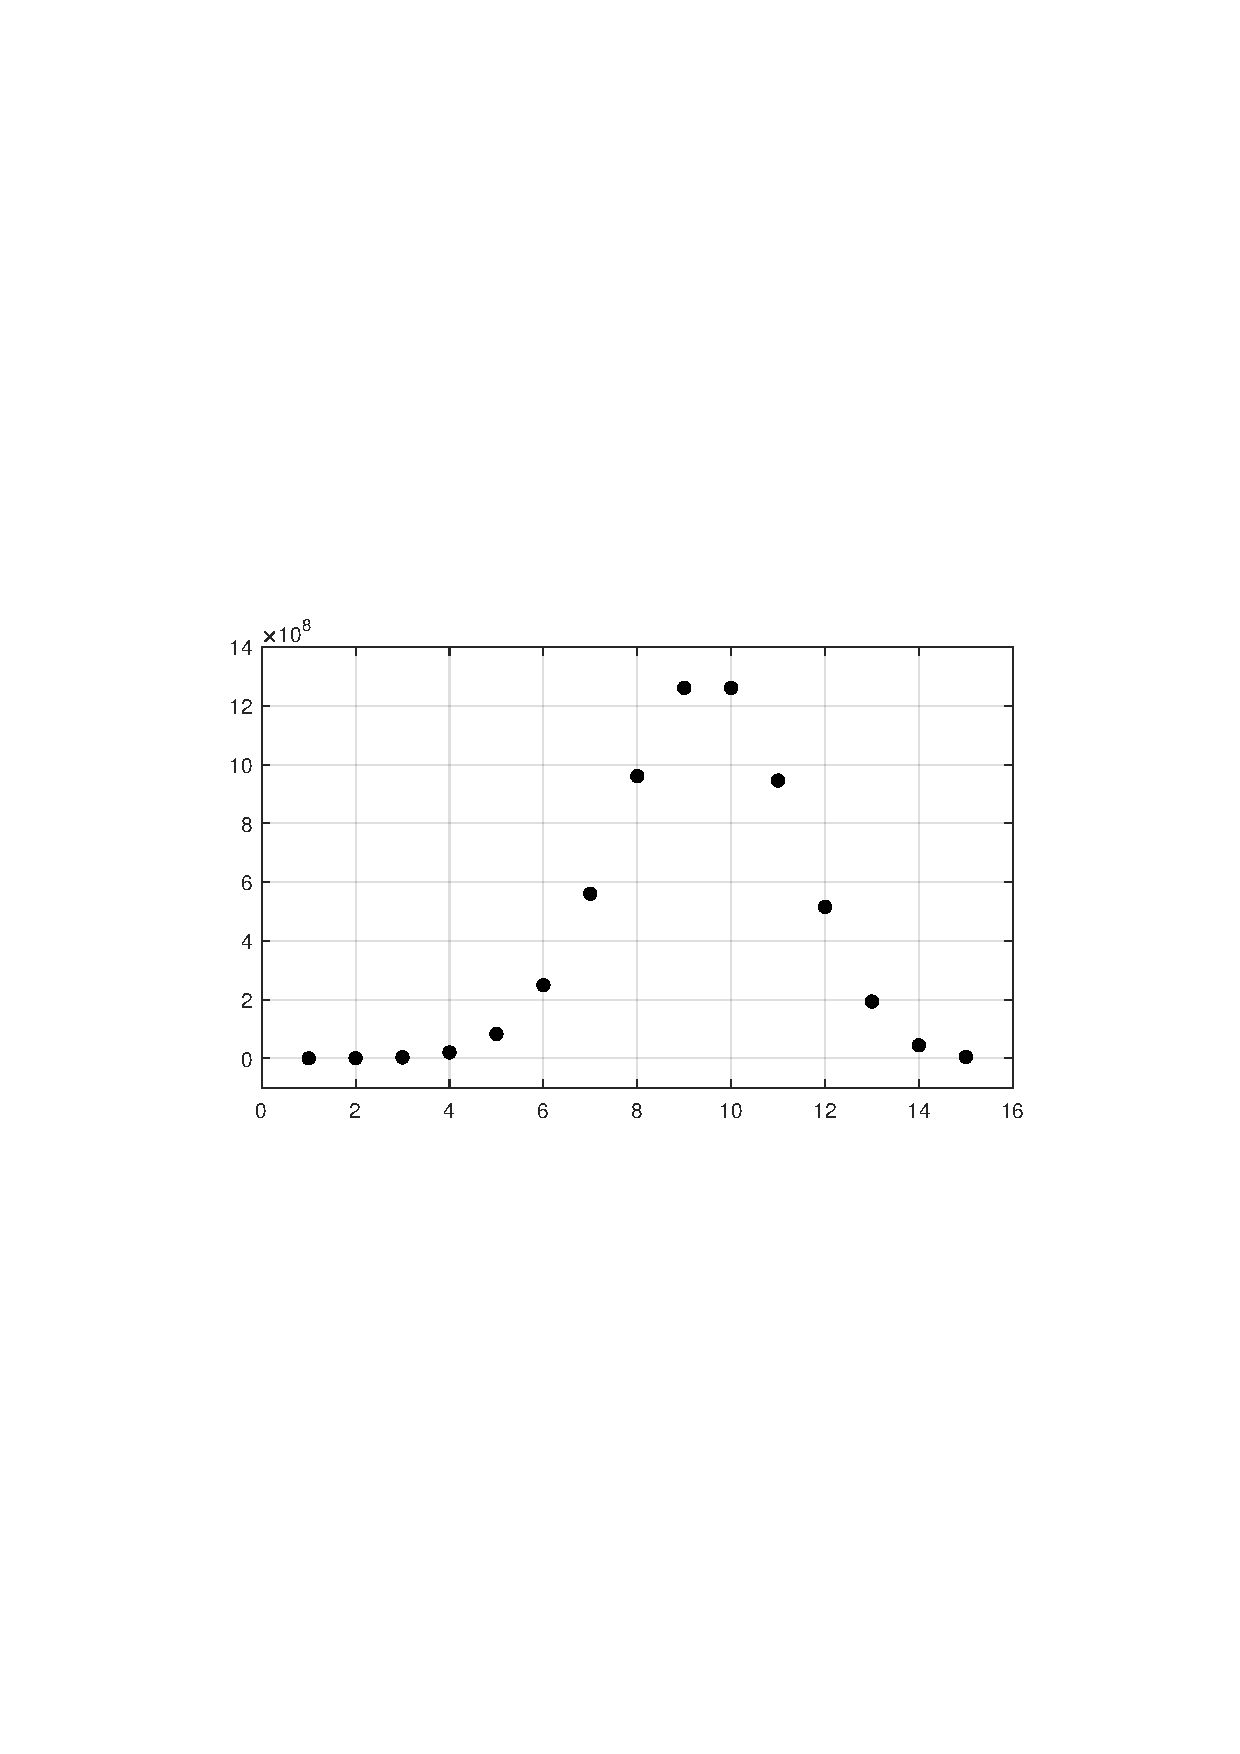
\includegraphics[width=0.4\linewidth]{二项式系数最大2}
\end{figure}
系数最大的有两项:$ C_{14}^{8}(2x)^6(3)^8=1260971712x^{6},\ 
C_{14}^{9}(2x)^5(3)^9=1260971712x^{5} $

\item 略

\item 30的因数有$ 1,2,3,5,6,10,15,30 $,从这8个因数每次取2个,不同比例的组合有\\
$ (1,1) $,$ (1,2) $,$ (1,3) $,$ (1,5) $,$ (1,6) $,$(1,10)$,
$ (1,15) $, $(1,30)$,\\
$ (2,3) $,$(2,5)$,$(2,15)$,\\
$ (3,5) $, $(3,10)$,\\
$ (5,6) $,\\
总共14种。

\item (1) 个位为0时,有$P_6^3=120$种;\\
个位为$2,4,6$时,因为0不能出现在首位,首位有5种选择。
有$ 3\times 5 \times 5 \times 4= 300 $种;\\
一共420种。\\
(2) $0+1+2+3+4+5+6=21$,能被3整除的数,各位数字之和也能被3整除,
$ 0\sim 6 $这7个数的和为21,恰好能被3整除,从中选5个数,
意味着剩余2个数字之和也要能被3整除,有如下可能
$ 0+3,\ 0+6,\ 1+2,\ 1+5,\ 2+4,\ 3+6,\ 4+5 $.\\
剩余$0+3,\ 0+6$时,有$2P_5^5=240$种;\\
剩余$1+2,\ 1+5,\ 2+4,\ 3+6,\ 4+5 $时,有$5\times4 P_4^4=480$种;\\
一共720种。\\
(3) 可构成的最小的6位数是$ 102345 $,以10开头的6位数,一共有
$P_5^4=120$个,这120个数中,最大的数为$106543$,从大到小的第21个,
就是从小到大的第100个。以106开头的6位数,一共有
$P_4^3=24 $种,这24个数从小到大为$106234,\ 106235,
\ 106243,\ 106245 $,第4个数106245便是最终结果。

\item \textbf{方法一}\ 
(1)使用2张10元,有$ 5+1 $,$ 2\times 3 $,
$ 2\times 2+1\times 2 $,$ 2\times 1+1\times 4 $,
$ 1\times 6 $,共5种。\\
(2)使用1张10元,至少2张5元,方法数与(1)相同,共5种。\\
(3)使用1张10元,若使用1张5元,2元的数量从5递减到0,共6种;
若使用0张5元,2元的数量从8递减到0,共9种;\\
(4)不使用10元,5张5元,共1种;4张5元,2元的数量从3递减到0,共4种;
3张5元,2元的数量从5递减到0,共6种;2张5元,2元的数量从8递减到0,共9种;
1张5元,2元的数量从10递减到0,共11种;0张5元,2元的数量从13递减到0,共14种;\\
综合以上,一共有$ 5+5+6+9+1+4+6+9+11+14=70 $种方法。\\
\textbf{方法二}$ ^* $\ 生成函数法,
\begin{gather*}
    \dfrac{1}{(1-x^1)(1-x^2)(1-x^{5})(1-x^{10})}=\\
    1+x+2x^{2}+2x^{3}+3x^{4}+4x^{5}+5x^{6}+6x^{7}+7x^{8}+8x^{9}+11x^{10}+12x^{11}+15x^{12}\\ +16x^{13}+19x^{14}+22x^{15}+25x^{16}+28x^{17}+31x^{18}+34x^{19}+40x^{20}+43x^{21}+49x^{22}\\
    +52x^{23}+58x^{24}+64x^{25}+70x^{26}+\cdots
\end{gather*}
凑出26元的方法数就等于$ x^{26} $的系数70. 
 
\end{enumerate}
\myfootnote{\CopyrightStatementChap}
% {\footnotesize (可在以下空白区域自行增补知识点。)}  
\cleardoublepage

%~\newpage
%~\newpage
%------------------------------------------
